%%%%%%%%%%%%%%%%%%%%%%%%%%%%%%%% Algoritmo:

\begin{frame}[fragile]{Algoritmo:}{Finalización.}
  Los índices conglomerador, que deben fusionarse se ajustan durante la fase de finalización.

  La estructura de datos, que almacena los índices de los grupos es una matriz de listas.
  \begin{figure}
    \centering
    \begin{subfigure}[b]{0.6\textwidth}
      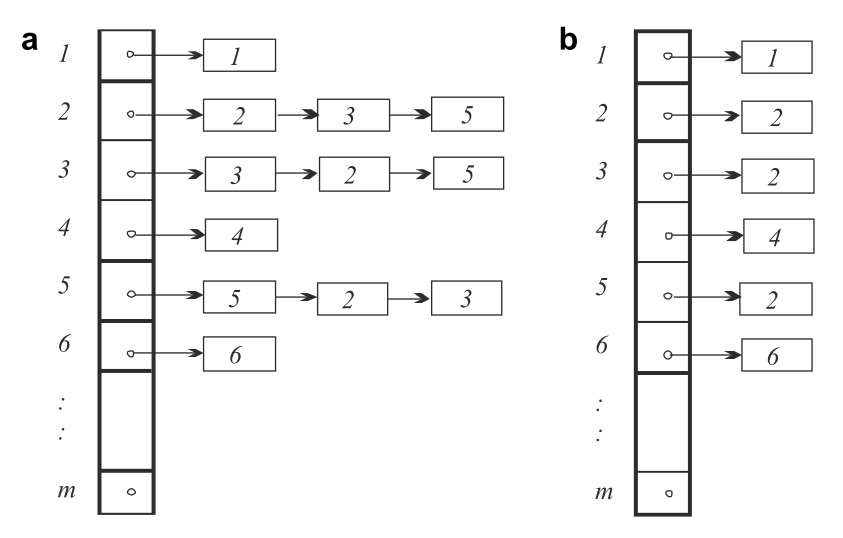
\includegraphics[width=\textwidth]{./Imagenes/FusionConglomerados.png}
      \caption*{Estructura auxiliar.}
    \end{subfigure}
  \end{figure}
  En cada lista se conserva el registro que tiene el valor de índices más pequeño, mientras se eliminan.
\end{frame}
